\documentclass[conference]{IEEEtran}
% FairLens -- IEEE conference paper, formatted to match the group's Eco-Shield paper.
% Build: `tectonic main.tex` (or pdflatex + bibtex) from paper/.
% All numbers come from data/verified_benchmark_results.json and paper/paper_stats.json.

\usepackage{newtxtext,newtxmath}
\usepackage{cite}
\usepackage{amsmath}
\usepackage{graphicx}
\usepackage{textcomp}
\usepackage{xcolor}
\usepackage{multirow}
\usepackage{array}
\usepackage{tikz}
\usetikzlibrary{positioning,arrows.meta,shapes.misc}
\usepackage[hidelinks]{hyperref}
\usepackage{balance}

\newcommand{\eps}{\varepsilon}
\newcommand{\DP}{\mathrm{DP}}
\newcommand{\EO}{\mathrm{EO}}
% Second row of author blocks in IEEEtran conference mode
\makeatletter
\newcommand{\linebreakand}{%
  \end{@IEEEauthorhalign}\hfill\mbox{}\par
  \mbox{}\hfill\begin{@IEEEauthorhalign}}
\makeatother
% Figure palette (matches the Eco-Shield paper's pastel boxes)
\definecolor{boxblue}{RGB}{219,232,246}
\definecolor{edgeblue}{RGB}{52,82,122}
\definecolor{boxpeach}{RGB}{250,226,206}
\definecolor{edgepeach}{RGB}{150,90,45}
\definecolor{boxsand}{RGB}{252,240,205}

\begin{document}

\title{FairLens: A Reproducible Framework for Auditing and Mitigating Demographic Bias in Tabular Classifiers, Evaluated on Three Benchmarks}

% Fixed-width author blocks so every column has the same width and both rows line up.
\newcommand{\authorbox}[2]{\parbox[t]{0.29\textwidth}{\centering
  {\normalsize\upshape #1}\\[2pt]
  {\small\itshape Department of Computer Engineering}\\
  {\small\itshape Vishwakarma Institute of Technology,}\\
  {\small\upshape Pune 411 037, Maharashtra, India}\\
  {\small\upshape #2}}}
\author{\IEEEauthorblockA{\begin{minipage}{\textwidth}\centering
\authorbox{Kapil Netaji Vhatkar\textsuperscript{*}}{kapilnv@gmail.com}\hspace{0.035\textwidth}%
\authorbox{Prachi Dilip Waghmare}{prachiwaghmare2206@gmail.com}\hspace{0.035\textwidth}%
\authorbox{Arnav Tibdewal}{arnavtibdewal19@gmail.com}\\[12pt]
\authorbox{Vihan Saraf}{vihanrsaraf@gmail.com}\hspace{0.035\textwidth}%
\authorbox{Eshwari Pravin Wasankar}{wasankareshwari@gmail.com}\hspace{0.035\textwidth}%
\parbox[t]{0.29\textwidth}{\mbox{}}
\end{minipage}}}

\maketitle
{\renewcommand{\thefootnote}{}\footnotetext{\textsuperscript{*}Corresponding author.}}

\begin{abstract}
FairLens is an open-source tool for auditing binary classifiers on tabular data for group bias. Given a dataset, a model and a protected attribute, it reports four fairness gaps (demographic parity, equalized odds, equal opportunity and predictive parity) with bootstrap intervals, ranks proxy features by mutual information, runs Reweighing, Exponentiated Gradient and Threshold Optimizer, and explains single predictions with SHAP and DiCE. None of these algorithms is ours. What we contribute is the plumbing around them (leakage removal, significance testing, tolerance tuning and label handling), which in our experience is where audits quietly go wrong. Results are reported for German Credit, COMPAS and Adult Income, each over ten random splits. Threshold Optimizer and Exponentiated Gradient lowered the COMPAS demographic parity gap by 0.216 and 0.208 respectively, both significant under a paired bootstrap, although Exponentiated Gradient gave up 8.4 accuracy points to do it against 2.3 for Threshold Optimizer. On Adult Income the same two methods closed the parity gap and opened up the equalized odds gap. The COMPAS baseline was about as well calibrated for African-American defendants as for Caucasian defendants (ECE 0.027 vs.\ 0.029) while selecting them at rates 0.24 apart, and its race$\times$sex gap of 0.368 exceeded both single-attribute gaps. We also list seven bugs from our own first implementation; one of them inflated a reported disparity by a factor of 2.9.
\end{abstract}

\begin{IEEEkeywords}
Algorithmic Fairness, Bias Mitigation, Bootstrap Inference, Calibration, Intersectionality, Explainable AI, Reproducibility
\end{IEEEkeywords}

%=====================================================================
\section{Introduction}\label{sec:intro}
%=====================================================================
In 2016 ProPublica reported that COMPAS, a risk score used by courts in Broward County, Florida, flagged African-American defendants who never reoffended as high risk far more often than Caucasian defendants who never reoffended~\cite{angwin2016machine}. The vendor answered that the score was equally calibrated for both groups. Both statements held up. Chouldechova~\cite{chouldechova2017fair} and Kleinberg et al.~\cite{kleinberg2017inherent} then showed that this tension is unavoidable whenever base rates differ: a score cannot be calibrated and have equal error rates across groups at the same time. A claim that a model is ``fair'' therefore has to say which definition it uses, and an audit is more useful when it reports several.

Most of the machinery already exists. Hardt et al.~\cite{hardt2016equality} introduced equalized odds and equal opportunity together with a post-processing fix based on group thresholds. Reweighing~\cite{kamiran2012data} acts before training, and the reductions approach of Agarwal et al.~\cite{agarwal2018reductions} adds a fairness constraint during training. Fairlearn~\cite{bird2020fairlearn} packages most of this, while SHAP~\cite{lundberg2017unified} and DiCE~\cite{mothilal2020explaining} cover feature attributions and counterfactual recourse. Kearns et al.~\cite{kearns2018preventing} added a warning that matters for auditing: a model can pass separate checks on sex and on race and still treat, for instance, women of one race unfairly.

We started FairLens as a dashboard on top of these libraries and expected the metrics to be the hard part. They were not. Almost every wrong number we produced came from somewhere else: a column that leaked the label, a tolerance tuned on the test set, a significance rule that could never return ``not significant'', or code that assumed label~1 was the good outcome. Each of these still yields a plausible number, which is why they are easy to miss. FairLens now records these choices in a configuration file and checks them with automated tests (52 at the time of writing).

This paper describes the tool and what it found on three public datasets, and also lists what we got wrong on the way. Its contributions are (i) a layered design in which the dashboard and the batch scripts share the same analysis code and the same results file, (ii) an evaluation protocol built on full-sample point estimates, signed-gap significance tests, paired tests for mitigation and validation-only tuning of the tolerance $\eps$, and (iii) results on German Credit, COMPAS and Adult Income, together with seven pipeline errors and their fixes.

It should be noted that the paired bootstrap tests are done on one split only and that German Credit has just 200 test rows. The significance results are therefore about these benchmarks and should not be taken as a guarantee for a model used in practice.

%=====================================================================
\section{Methodology}\label{sec:method}
%=====================================================================
\subsection{System Overview and Architecture}
FairLens is written in Python using pandas, scikit-learn, XGBoost, Fairlearn~\cite{bird2020fairlearn}, SHAP and DiCE. It has four layers, shown in Fig.~\ref{fig:sysarch}. The \emph{persistence} layer is at the bottom and stores a YAML file that configures each dataset, the raw data files, a JSON results file, the trained models and a SQLite log of earlier runs. The \emph{core} layer has six packages: data, analysis, models, fairness, explainability and reporting. These packages only pass data frames and a small object containing the train, validation and test splits and the fitted scaler between each other, and none of them depends on the user interface. This let us use the same code in the dashboard, in the batch evaluation, in the unit tests, and in the scripts that made the tables and figures for this paper.

\begin{figure*}[t]
\centering
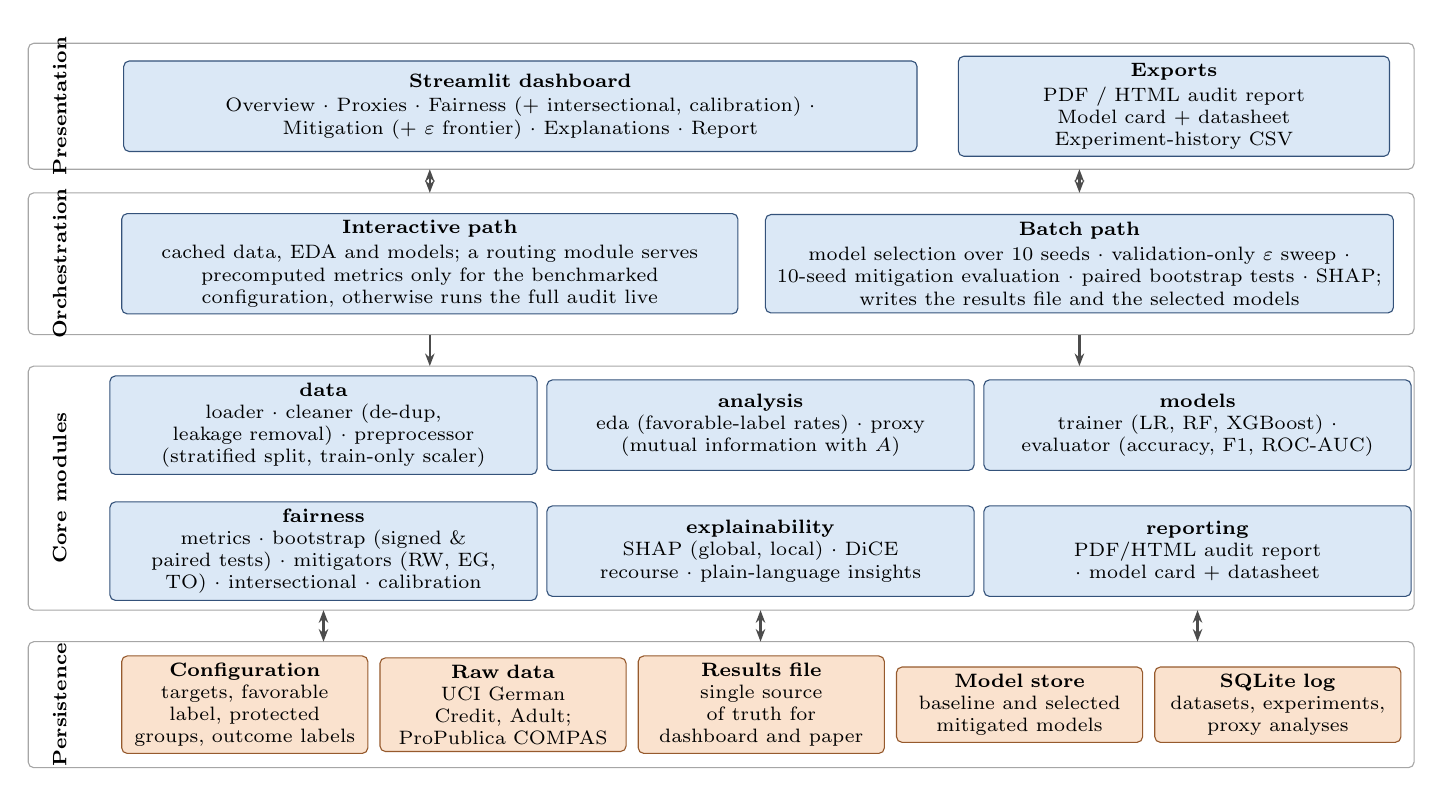
\begin{tikzpicture}[
  font=\scriptsize,
  mod/.style={execute at begin node={\hyphenpenalty=10000\exhyphenpenalty=10000}, draw=edgeblue, fill=boxblue, rounded corners=2pt, align=center, inner sep=2.5pt, text width=#1},
  mod/.default=5.25cm,
  store/.style={execute at begin node={\hyphenpenalty=10000\exhyphenpenalty=10000}, draw=edgepeach, fill=boxpeach, rounded corners=2pt, align=center, inner sep=2.5pt, text width=2.95cm, minimum height=0.95cm},
  lab/.style={rotate=90, font=\scriptsize\bfseries, anchor=center},
  arr/.style={-{Stealth[length=1.6mm]}, thick, black!70},
  darr/.style={{Stealth[length=1.6mm]}-{Stealth[length=1.6mm]}, thick, black!70}]

\draw[black!35, rounded corners=2pt] (0,9.35) rectangle (17.6,10.95);
\node[lab] at (0.4,10.15) {Presentation};
\node[mod=9.9cm, minimum height=1.15cm] (dash) at (6.25,10.15) {\textbf{Streamlit dashboard}\\[1pt]
  Overview $\cdot$ Proxies $\cdot$ Fairness (+ intersectional, calibration) $\cdot$\\
  Mitigation (+ $\varepsilon$ frontier) $\cdot$ Explanations $\cdot$ Report};
\node[mod=5.3cm, minimum height=1.15cm] (exp) at (14.55,10.15) {\textbf{Exports}\\[1pt] PDF / HTML audit report\\ Model card + datasheet\\ Experiment-history CSV};

\draw[black!35, rounded corners=2pt] (0,7.25) rectangle (17.6,9.05);
\node[lab] at (0.4,8.15) {Orchestration};
\node[mod=7.65cm, minimum height=1.25cm] (inter) at (5.1,8.15) {\textbf{Interactive path}\\[1pt]
  cached data, EDA and models; a routing module serves\\ precomputed metrics only for the benchmarked\\ configuration, otherwise runs the full audit live};
\node[mod=7.8cm, minimum height=1.25cm] (batch) at (13.35,8.15) {\textbf{Batch path}\\[1pt]
  model selection over 10 seeds $\cdot$ validation-only $\varepsilon$ sweep $\cdot$\\
  10-seed mitigation evaluation $\cdot$ paired bootstrap tests $\cdot$ SHAP;\\ writes the results file and the selected models};

\draw[black!35, rounded corners=2pt] (0,3.75) rectangle (17.6,6.85);
\node[lab] at (0.4,5.3) {Core modules};
\node[mod, minimum height=1.15cm] (data) at (3.75,6.1) {\textbf{data}\\ loader $\cdot$ cleaner (de-dup, leakage removal) $\cdot$ preprocessor (stratified split, train-only scaler)};
\node[mod, minimum height=1.15cm] (anal) at (9.3,6.1) {\textbf{analysis}\\ eda (favorable-label rates) $\cdot$ proxy (mutual information with $A$)};
\node[mod, minimum height=1.15cm] (mdl) at (14.85,6.1) {\textbf{models}\\ trainer (LR, RF, XGBoost) $\cdot$ evaluator (accuracy, F1, ROC-AUC)};
\node[mod, minimum height=1.15cm] (fair) at (3.75,4.5) {\textbf{fairness}\\ metrics $\cdot$ bootstrap (signed \& paired tests) $\cdot$ mitigators (RW, EG, TO) $\cdot$ intersectional $\cdot$ calibration};
\node[mod, minimum height=1.15cm] (xai) at (9.3,4.5) {\textbf{explainability}\\ SHAP (global, local) $\cdot$ DiCE recourse $\cdot$ plain-language insights};
\node[mod, minimum height=1.15cm] (rep) at (14.85,4.5) {\textbf{reporting}\\ PDF/HTML audit report $\cdot$ model card + datasheet};

\draw[black!35, rounded corners=2pt] (0,1.75) rectangle (17.6,3.35);
\node[lab] at (0.4,2.55) {Persistence};
\node[store] (cfg) at (2.75,2.55) {\textbf{Configuration}\\ targets, favorable label, protected groups, outcome labels};
\node[store] (raw) at (6.03,2.55) {\textbf{Raw data}\\ UCI German Credit, Adult; ProPublica COMPAS};
\node[store] (json) at (9.31,2.55) {\textbf{Results file}\\ single source of truth for dashboard and paper};
\node[store] (jl) at (12.59,2.55) {\textbf{Model store}\\ baseline and selected mitigated models};
\node[store] (db) at (15.87,2.55) {\textbf{SQLite log}\\ datasets, experiments, proxy analyses};

\draw[darr] (5.1,9.35) -- (5.1,9.05);
\draw[darr] (13.35,9.35) -- (13.35,9.05);
\draw[arr] (5.1,7.25) -- (5.1,6.85);
\draw[arr] (13.35,7.25) -- (13.35,6.85);
\draw[darr] (3.75,3.75) -- (3.75,3.35);
\draw[darr] (9.3,3.75) -- (9.3,3.35);
\draw[darr] (14.85,3.75) -- (14.85,3.35);
\end{tikzpicture}
\caption{FairLens system architecture. Two execution paths share the same core modules: the batch path computes the ten-seed benchmark and stores it in a single results file; the interactive dashboard serves those results for the benchmarked configuration and recomputes everything live for any other dataset, model or protected attribute.}
\label{fig:sysarch}
\end{figure*}

The \emph{orchestration} layer has two paths for running an audit. The batch path runs model selection, the $\eps$ sweep and the evaluation over ten seeds, and writes all the numbers reported in this paper into the results file. The interactive path runs the full audit when the user asks for it, which is needed whenever a user uploads their own data or picks a model and attribute combination that was never benchmarked. A live run is not instant; on our development machine a complete audit of Adult Income took between 47 and 87 seconds depending on the model and attribute, so stored results are reused where that is safe. A routing module makes that decision, and stored results are shown only if the user's selection is exactly the benchmarked one (see P6 in Section~\ref{sec:pitfalls}). The \emph{presentation} layer is a Streamlit dashboard with six tabs (Overview, Proxies, Fairness, Mitigation, Explanations and Report) that follow the stages of the pipeline in Fig.~\ref{fig:arch}; it can also export a PDF report and a model card with a datasheet. Four of these tabs are shown in Fig.~\ref{fig:ui} for German Credit. The dataset, protected attribute and model are chosen in the sidebar, every disparity card shows the signed interval and whether the gap is significant, and the outcome names come from the dataset configuration.

\begin{figure*}[t]
\centering
\setlength{\fboxsep}{0pt}\setlength{\fboxrule}{0.4pt}
\begin{minipage}[t]{0.49\textwidth}\centering
\fbox{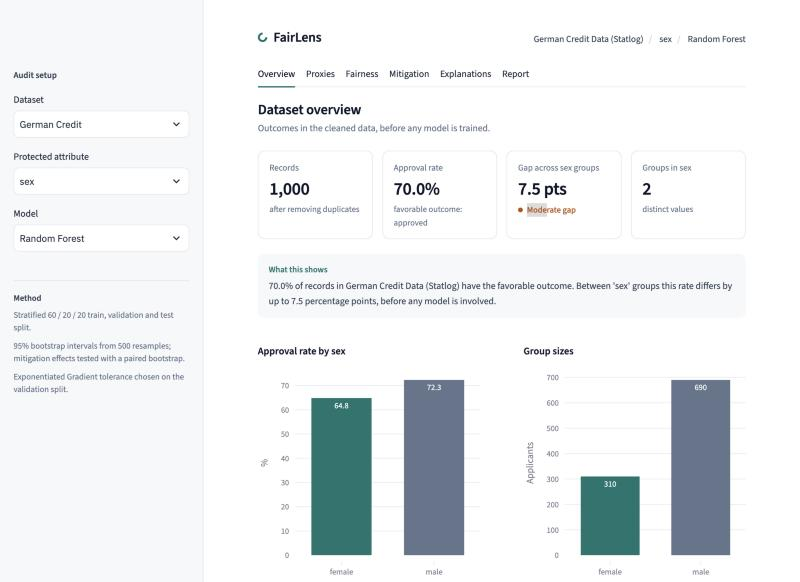
\includegraphics[width=\dimexpr\linewidth-0.8pt\relax]{figures/ui_overview.jpg}}\\[2pt]
{\footnotesize (a) Overview: dataset summary and base-rate gap}
\end{minipage}\hfill
\begin{minipage}[t]{0.49\textwidth}\centering
\fbox{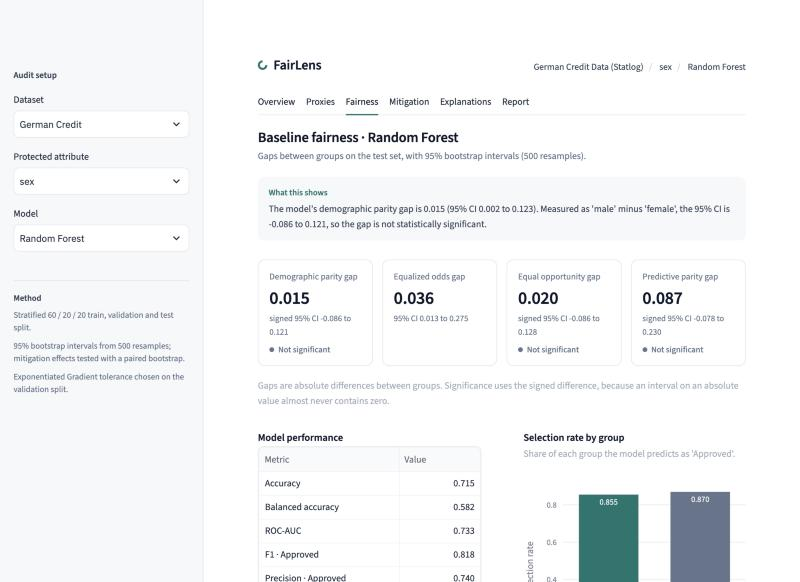
\includegraphics[width=\dimexpr\linewidth-0.8pt\relax]{figures/ui_fairness.jpg}}\\[2pt]
{\footnotesize (b) Fairness: point estimates, signed intervals and significance}
\end{minipage}\\[6pt]
\begin{minipage}[t]{0.49\textwidth}\centering
\fbox{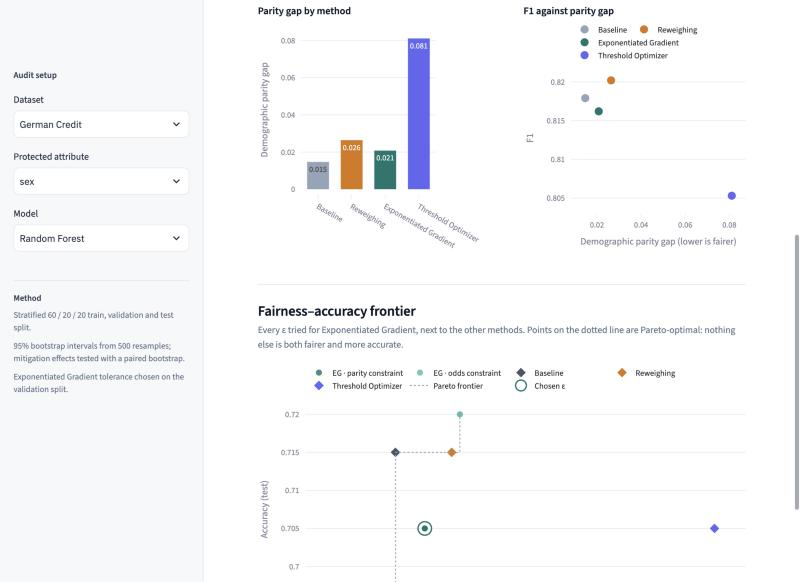
\includegraphics[width=\dimexpr\linewidth-0.8pt\relax]{figures/ui_mitigation.jpg}}\\[2pt]
{\footnotesize (c) Mitigation: method comparison and $\varepsilon$ frontier}
\end{minipage}\hfill
\begin{minipage}[t]{0.49\textwidth}\centering
\fbox{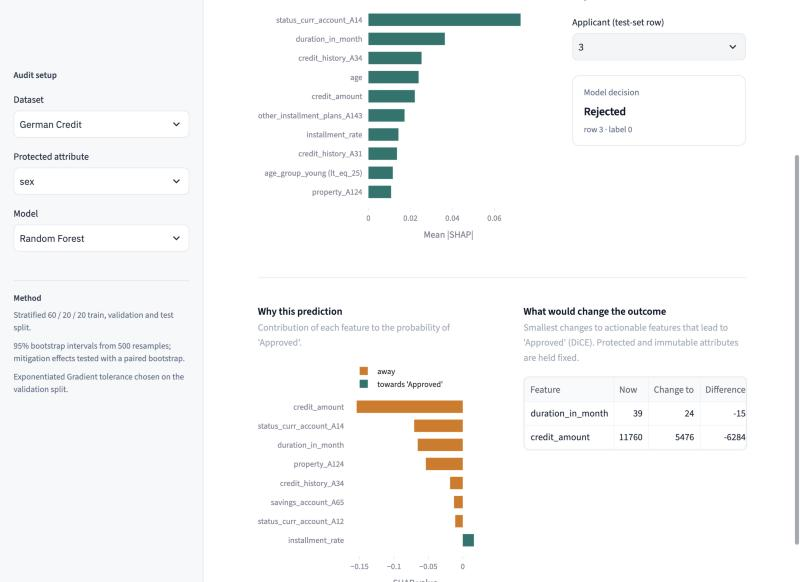
\includegraphics[width=\dimexpr\linewidth-0.8pt\relax]{figures/ui_explanations.jpg}}\\[2pt]
{\footnotesize (d) Explanations: SHAP attributions and DiCE recourse}
\end{minipage}
\caption{FairLens dashboard on German Credit (protected attribute sex, Random Forest baseline). Each tab mirrors one stage of the audit pipeline in Fig.~\ref{fig:arch}.}
\label{fig:ui}
\end{figure*}
\begin{figure}[t]
\centering
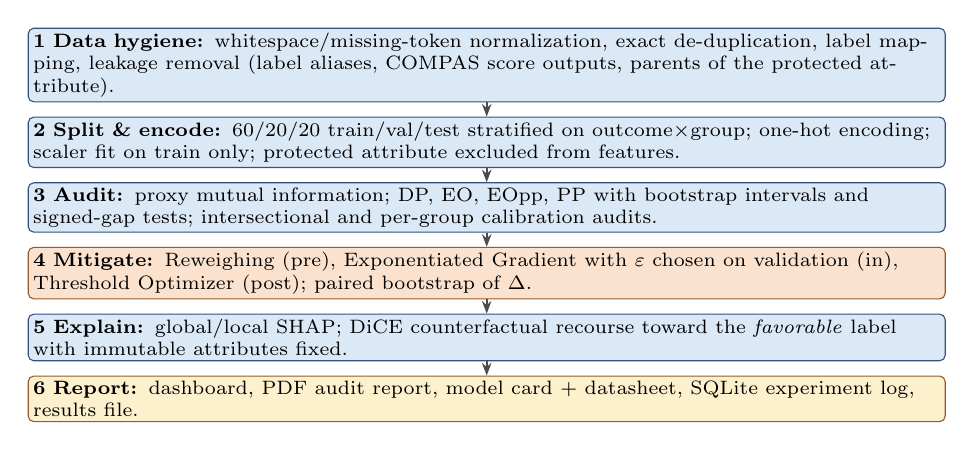
\begin{tikzpicture}[
  node distance=1.8mm,
  box/.style={rectangle, rounded corners=2pt, draw=edgeblue, fill=#1, text width=0.95\columnwidth, align=left, inner sep=1.8pt, font=\scriptsize},
  box/.default=boxblue,
  arr/.style={-{Stealth[length=1.6mm]}, thick, black!70}]
\node[box] (d) {\textbf{1 Data hygiene:} whitespace/missing-token normalization, exact de-duplication, label mapping, leakage removal (label aliases, COMPAS score outputs, parents of the protected attribute).};
\node[box, below=of d] (p) {\textbf{2 Split \& encode:} 60/20/20 train/val/test stratified on outcome$\times$group; one-hot encoding; scaler fit on train only; protected attribute excluded from features.};
\node[box, below=of p] (a) {\textbf{3 Audit:} proxy mutual information; DP, EO, EOpp, PP with bootstrap intervals and signed-gap tests; intersectional and per-group calibration audits.};
\node[box=boxpeach, draw=edgepeach, below=of a] (m) {\textbf{4 Mitigate:} Reweighing (pre), Exponentiated Gradient with $\eps$ chosen on validation (in), Threshold Optimizer (post); paired bootstrap of $\Delta$.};
\node[box, below=of m] (e) {\textbf{5 Explain:} global/local SHAP; DiCE counterfactual recourse toward the \emph{favorable} label with immutable attributes fixed.};
\node[box=boxsand, draw=edgepeach, below=of e] (r) {\textbf{6 Report:} dashboard, PDF audit report, model card + datasheet, SQLite experiment log, results file.};
\foreach \u/\v in {d/p,p/a,a/m,m/e,e/r} \draw[arr] (\u) -- (\v);
\end{tikzpicture}
\caption{FairLens audit pipeline. Every number shown in the dashboard or in this paper is produced by stages 1--6 and stored in a single results file.}
\label{fig:arch}
\end{figure}

\subsection{Benchmark Datasets}
\subsubsection{Why these benchmarks} We used German Credit (Statlog) and Adult Income from the UCI Machine Learning Repository and the two-year COMPAS file released by ProPublica~\cite{angwin2016machine}. These three datasets are public and are used in most fairness papers, so our numbers can be compared with earlier work, and they cover three different areas, namely credit, criminal justice and income. COMPAS is useful for one more reason. Label~1 there means that the person reoffended, which is the \emph{unfavorable} outcome, so it tests whether FairLens really takes the favorable label from the configuration rather than assuming that 1 is good. Some known issues with these datasets, mainly label bias and their age, are discussed in Section~\ref{sec:limits}.

\subsubsection{Dataset partitions} As in the original analysis~\cite{angwin2016machine}, only COMPAS records with $|\texttt{days\_b\_screening\_arrest}|\le 30$ are kept. Every dataset is split 60/20/20 into training, validation and test sets, stratified on outcome and protected group together, and each experiment is repeated for ten splits (seeds 42--51). The cleaned datasets are summarized in Table~\ref{tab:data}. The bootstrap intervals, paired tests, $\eps$ sweep and the intersectional and calibration audits are all done on the seed-42 split.

\begin{table}[t]
\centering
\caption{Benchmark Datasets After Cleaning}
\label{tab:data}
\setlength{\tabcolsep}{3pt}
\renewcommand{\arraystretch}{1.12}
\resizebox{\columnwidth}{!}{%
\begin{tabular}{|l|c|c|c|}
\hline
\textbf{Property} & \textbf{German Credit} & \textbf{COMPAS} & \textbf{Adult Income} \\
\hline
Rows raw $\to$ clean & 1{,}000 $\to$ 1{,}000 & 7{,}214 $\to$ 6{,}172 & 32{,}561 $\to$ 32{,}537 \\
Encoded features & 46 & 10 & 97 \\
Train / val / test & 600/200/200 & 3703/1234/1235 & 19522/6507/6508 \\
Protected attribute & sex & race & sex \\
Privileged / unpriv. & male / female & Cauc. / Afr.-Am. & male / female \\
Favorable outcome & good credit & no recidivism & income $>$\$50K \\
Favorable rate & 70.0\% & 54.5\% & 24.1\% \\
\quad privileged & 72.3\% & 60.9\% & 30.6\% \\
\quad unprivileged & 64.8\% & 47.7\% & 11.0\% \\
\hline
\end{tabular}}
\end{table}

\subsection{Leakage Control and Proxy Analysis}
\subsubsection{Leakage control} For every dataset there is a configuration file listing the target column and its favorable value, the protected attributes and their privileged groups, the features that cannot be changed (needed by DiCE), and the text used for each outcome. In cleaning, exact duplicate rows are removed and the target is mapped to $\{0,1\}$. After this, three types of leakage are removed. First, any other column that encodes the label is dropped. Second, for COMPAS, the outputs of the COMPAS tool itself (\texttt{decile\_score}, \texttt{score\_text} and similar fields) and fields recorded after the outcome are dropped, since a model trained on the COMPAS score would just learn to copy it. Third, if a protected attribute was created from another column, like \texttt{sex} from \texttt{personal\_status\_sex} in German Credit, that column is also dropped. The protected attribute is never given to the model as an input.

\subsubsection{Proxy analysis} Removing the protected attribute $A$ from the inputs does not mean the model cannot learn it from other features. To check this we compute the mutual information $I(X_j;A)$ between $A$ and each feature $X_j$ and rank the features by this value.

\subsection{Fairness Metrics and Statistical Inference}
Let $\hat{Y}\in\{0,1\}$ be the prediction, $Y$ the label and $A$ the protected attribute with privileged group $p$ and unprivileged group $u$. With selection rate $\mathrm{SR}_g=P(\hat{Y}{=}1\mid A{=}g)$ and $\mathrm{TPR}_g,\mathrm{FPR}_g,\mathrm{PPV}_g$ defined as usual,
\begin{align}
\DP &= |\mathrm{SR}_p-\mathrm{SR}_u|,\\
\EO &= \max\big(|\mathrm{TPR}_p-\mathrm{TPR}_u|,\;|\mathrm{FPR}_p-\mathrm{FPR}_u|\big),\\
\mathrm{EOpp} &= |\mathrm{TPR}_p-\mathrm{TPR}_u|,\qquad \mathrm{PP}=|\mathrm{PPV}_p-\mathrm{PPV}_u|.
\end{align}
For attributes with more than two groups and no designated pair, gaps are max--min over groups with at least 30 test members. ``Selection'' refers to label~1; for COMPAS this is \emph{predicted recidivism}.

\subsubsection{Point estimates} Each metric is reported as its value on the complete test set, along with a 95\% percentile bootstrap interval using $B=500$ resamples. For test sets bigger than 3{,}000 rows, 3{,}000 rows are subsampled first. We do not use the mean of the bootstrap samples as the estimate, because for an absolute gap $|\theta|$ this mean is biased upwards and the bias is worst when the real gap is near zero (Section~\ref{sec:pitfalls}).

\subsubsection{Signed-gap significance} Since an interval for $|\theta|$ almost never contains zero, it cannot be used to show that a gap is absent. So we first fix the reference pair $(a,b)$ on the full sample such that $\hat\theta=\mathrm{SR}_a-\mathrm{SR}_b\ge 0$, then bootstrap the \emph{signed} difference, and a gap is called significant only if this interval does not contain zero. The same is done for EOpp and PP.

\subsubsection{Paired mitigation test} For testing a mitigation method we bootstrap $\Delta=\DP_{\text{base}}-\DP_{\text{mit}}$ using the \emph{same} resampled rows for both models ($B=500$). If the 95\% interval of $\Delta$ lies completely above zero, the reduction is taken as significant. Using the same rows for both models removes most of the sampling noise from the comparison.

\subsection{Models and Mitigation}
We trained three types of models: logistic regression (LR; $C{=}1$, on standardized features), random forest (RF; 100 trees, depth 8) and XGBoost (100 trees, depth 5, learning rate 0.1). For every dataset the model type with the highest mean validation F1 over the ten splits was used as the baseline (Table~\ref{tab:select}), which was RF for German Credit and COMPAS and XGBoost for Adult.

\begin{table}[t]
\centering
\caption{Baseline Model Selection: Validation F1 (Mean $\pm$ Std Over 10 Splits)}
\label{tab:select}
\renewcommand{\arraystretch}{1.12}
\footnotesize
\begin{tabular}{|l|c|c|c|}
\hline
\textbf{Dataset} & \textbf{LR} & \textbf{RF} & \textbf{XGBoost} \\
\hline
German Credit & 0.819 $\pm$ 0.015 & \textbf{0.837 $\pm$ 0.012} & 0.821 $\pm$ 0.016 \\
COMPAS & 0.614 $\pm$ 0.012 & \textbf{0.632 $\pm$ 0.016} & 0.625 $\pm$ 0.013 \\
Adult Income & 0.665 $\pm$ 0.009 & 0.622 $\pm$ 0.011 & \textbf{0.705 $\pm$ 0.009} \\
\hline
\end{tabular}
\end{table}

\subsubsection{Mitigation methods} Reweighing~\cite{kamiran2012data} trains the baseline model again with weights $w(a,y)=P(A{=}a)P(Y{=}y)/P(A{=}a,Y{=}y)$, so that $A$ and $Y$ become independent in the weighted training data. Exponentiated Gradient (EG)~\cite{agarwal2018reductions} minimizes the error while keeping the demographic parity gap within $\eps$ and gives a randomized mixture $Q$ of base classifiers. In our setup it uses 50 trees (depth 5 for RF and 3 for XGBoost) and 50 iterations. Threshold Optimizer (TO)~\cite{hardt2016equality} does not retrain the baseline; it learns one threshold per group on the validation split.

\subsubsection{Seeded randomized predictors} EG and TO give randomized predictions, and Fairlearn does not set a seed for them. We set a fixed seed and also return the positive-class probability of $Q$, so that all metrics of a model are calculated from the same predictions and ROC-AUC can be calculated.

\subsubsection{Validation-only selection of $\eps$} The values tried for $\eps$ are $\{0.005,0.01,0.02,0.05,0.1\}$. On the validation split, we first keep only the values for which accuracy drops by at most 5 percentage points (pp) from the baseline, and from these we choose the one with the lowest DP. If no value satisfies this, the value with the smallest drop in accuracy is chosen. The test split is not used anywhere in this selection.

\subsection{Intersectional, Calibration and Explanation Audits}
For two attributes $A$ and $C$, FairLens calculates SR, TPR and FPR for each cell $(a,c)$ and reports the difference between the highest and lowest value among cells having $n\ge30$. The single-attribute gaps computed on the same rows are shown beside it, so that gaps which exist only in subgroups~\cite{kearns2018preventing} can be noticed. For calibration, the Brier score, the expected calibration error $\mathrm{ECE}=\sum_k \frac{n_k}{n}|\bar{y}_k-\bar{p}_k|$ (10 equal-width bins) and a reliability curve with quantile bins are reported for each group. SHAP values are computed with TreeSHAP for the tree models and with a linear explainer for LR~\cite{lundberg2017unified}. For a person who gets the unfavorable prediction, DiCE~\cite{mothilal2020explaining} searches for counterfactuals that change the prediction while keeping the immutable attributes the same.

%=====================================================================
\section{Results and Discussion}\label{sec:results}
%=====================================================================
\subsection{Baseline Disparities}
On the seed-42 test split, the COMPAS baseline predicts recidivism much more often for African-American defendants than for Caucasian defendants, with a DP gap of 0.239 (signed 95\% interval [0.183, 0.292]). In Adult Income there is a gap of 0.163 in favor of men (interval [0.132, 0.182]). German Credit is a different case. The gap there is only 0.015 and the signed interval $[-0.086, 0.122]$ contains zero, so with a 200-row test set we cannot say that there is a disparity. Across the ten splits the baseline DP was $0.247\pm0.020$ for COMPAS, $0.173\pm0.006$ for Adult and $0.032\pm0.021$ for German Credit. When all COMPAS race groups with $n\ge30$ are considered, the max--min gap increases to 0.309.

\subsection{Mitigation Performance}
Table~\ref{tab:main} gives the results over the ten splits.

\begin{table*}[t]
\centering
\caption{Mitigation Results: Test Metrics as Mean $\pm$ Std Over 10 Splits; $\Delta\DP$ Is the Paired Bootstrap Reduction on the Seed-42 Split (95\% Interval). Bold: Interval Excludes Zero. F1 Refers to Label 1.}
\label{tab:main}
\renewcommand{\arraystretch}{1.12}
\footnotesize
\setlength{\tabcolsep}{5pt}
\begin{tabular}{|l|l|c|c|c|c|c|}
\hline
\textbf{Dataset (baseline)} & \textbf{Method} & \textbf{F1} & \textbf{Accuracy (\%)} & \textbf{DP} & \textbf{EO} & \textbf{$\Delta\DP$ [95\% interval]} \\
\hline
\multirow{4}{*}{German Credit (RF)}
 & Baseline & 0.829 $\pm$ 0.015 & 72.75 $\pm$ 2.24 & 0.032 $\pm$ 0.021 & 0.074 $\pm$ 0.030 & -- \\
 & Reweighing & 0.831 $\pm$ 0.010 & 72.95 $\pm$ 1.52 & 0.043 $\pm$ 0.030 & 0.087 $\pm$ 0.025 & $+0.000$ [$-0.080$, 0.092] \\
 & EG ($\eps{=}0.005$) & 0.829 $\pm$ 0.008 & 72.10 $\pm$ 1.11 & 0.033 $\pm$ 0.011 & 0.078 $\pm$ 0.055 & $+0.006$ [$-0.065$, 0.084] \\
 & Threshold Opt. & 0.828 $\pm$ 0.019 & 73.95 $\pm$ 3.22 & 0.048 $\pm$ 0.041 & 0.121 $\pm$ 0.073 & $-0.041$ [$-0.143$, 0.095] \\
\hline
\multirow{4}{*}{COMPAS (RF)}
 & Baseline & 0.634 $\pm$ 0.011 & 68.71 $\pm$ 0.79 & 0.247 $\pm$ 0.020 & 0.242 $\pm$ 0.032 & -- \\
 & Reweighing & 0.629 $\pm$ 0.009 & 68.35 $\pm$ 0.54 & 0.241 $\pm$ 0.020 & 0.232 $\pm$ 0.036 & $+0.002$ [$-0.014$, 0.016] \\
 & EG ($\eps{=}0.01$) & 0.400 $\pm$ 0.017 & 60.27 $\pm$ 0.64 & 0.059 $\pm$ 0.025 & 0.079 $\pm$ 0.049 & $\mathbf{+0.208}$ \textbf{[0.148, 0.259]} \\
 & Threshold Opt. & 0.606 $\pm$ 0.020 & 66.40 $\pm$ 1.14 & 0.027 $\pm$ 0.012 & 0.060 $\pm$ 0.024 & $\mathbf{+0.216}$ \textbf{[0.132, 0.268]} \\
\hline
\multirow{4}{*}{Adult Income (XGBoost)}
 & Baseline & 0.697 $\pm$ 0.006 & 86.85 $\pm$ 0.22 & 0.173 $\pm$ 0.006 & 0.094 $\pm$ 0.025 & -- \\
 & Reweighing & 0.681 $\pm$ 0.006 & 86.52 $\pm$ 0.26 & 0.093 $\pm$ 0.006 & 0.137 $\pm$ 0.026 & $\mathbf{+0.077}$ \textbf{[0.062, 0.092]} \\
 & EG ($\eps{=}0.1$) & 0.594 $\pm$ 0.012 & 84.31 $\pm$ 0.36 & 0.020 $\pm$ 0.007 & 0.258 $\pm$ 0.028 & $\mathbf{+0.142}$ \textbf{[0.121, 0.161]} \\
 & Threshold Opt. & 0.640 $\pm$ 0.011 & 85.02 $\pm$ 0.31 & 0.009 $\pm$ 0.006 & 0.310 $\pm$ 0.023 & $\mathbf{+0.144}$ \textbf{[0.106, 0.170]} \\
\hline
\end{tabular}
\end{table*}

For COMPAS, Reweighing made almost no difference ($\Delta=0.002$, interval contains zero). EG and TO removed most of the gap, with mean DP going down to 0.059 and 0.027, and EO also decreased. Between these two, TO is the better option for COMPAS since it lost only 2.3\,pp of accuracy against 8.4\,pp for EG. EG's F1 for label~1 also fell to 0.40, because the constrained model predicts recidivism much less often for all defendants.

For Adult Income, DP was reduced significantly by all three methods. Reweighing reduced it by about half with a 0.3\,pp loss in accuracy, while TO reduced it to 0.009 with a 1.8\,pp loss. However, men and women in Adult have base rates that differ by 19.6\,pp (Table~\ref{tab:data}), and forcing their selection rates to be equal moves their error rates apart. EO went up from 0.094 to 0.258 with EG and to 0.310 with TO, and on the seed-42 split both increases are significant ($\Delta\EO=-0.210$, interval $[-0.342,-0.039]$ for EG; $-0.263$, interval $[-0.379,-0.112]$ for TO). On Adult, in other words, demographic parity was bought at the expense of equalized odds.

For German Credit none of the methods gave a significant change and all the intervals contain zero. We expected this, as the baseline gap was also not significant.
\subsection{Fairness--Accuracy Frontier}
All the $\eps$ values we tried are plotted in Fig.~\ref{fig:frontier} for both the DP and EO constraints, along with the baseline and the other two methods. For German Credit, EG with the DP constraint gives exactly the same classifier for $\eps$ between 0.005 and 0.05, because the baseline already meets the constraint on the training data, and only $\eps=0.1$ gives a different one. For COMPAS, none of the $\eps$ values kept validation accuracy within 5\,pp of the baseline, and so the fallback rule selected $\eps=0.01$ (7.2\,pp loss on validation). For Adult all the values qualified and $\eps=0.1$ gave the lowest validation DP. On both COMPAS and Adult, TO is on the Pareto frontier of the test set while the EG points are dominated. This is possible because $\eps$ is chosen on validation data, and the selected EG point does not have to be the best one on the test set.

\begin{figure*}[t]
\centering
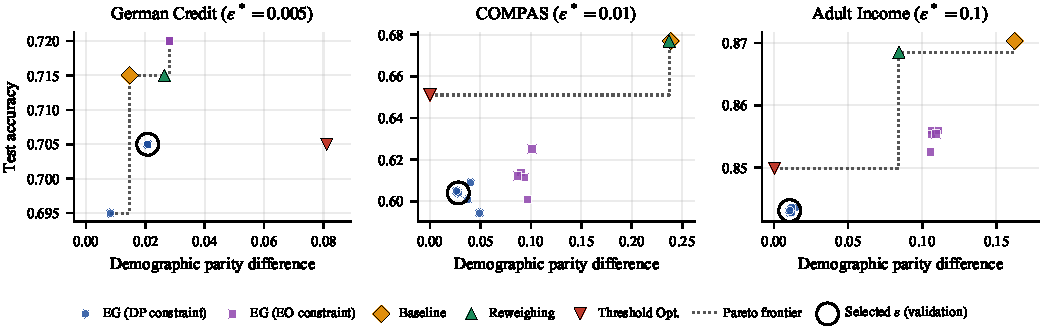
\includegraphics[width=\textwidth]{figures/frontier.pdf}
\caption{Fairness--accuracy trade-off on the seed-42 test split. Circles/squares: Exponentiated Gradient for each $\eps$ under DP/EO constraints; diamonds and triangles: baseline, Reweighing and Threshold Optimizer. Dotted line: Pareto frontier (lower DP and higher accuracy are better). The ringed point is the $\eps$ selected on the validation split.}
\label{fig:frontier}
\end{figure*}

\subsection{Intersectional Disparities}
Selection rates for all intersections with $n\ge30$ are shown in Fig.~\ref{fig:inter}. For COMPAS the race$\times$sex gap is 0.368, between African-American men with a predicted recidivism rate of 0.548 and Caucasian women with 0.179. This is larger than the race-only gap (0.309) as well as the sex-only gap (0.152), and false positive rates follow the same trend (0.350 vs.\ 0.141). For Adult the sex$\times$age gap is 0.284, while the gaps for sex and age group alone are 0.163 and 0.229. Prime-age men have a selection rate of 0.288 whereas for young women it is only 0.004. In German Credit, both of the ``young'' cells have less than 30 test applicants and are excluded. There is not enough data here for an intersectional result and FairLens reports this instead of giving an unstable number.

\begin{figure}[t]
\centering
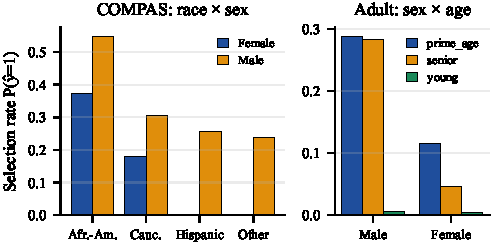
\includegraphics[width=\columnwidth]{figures/intersectional.pdf}
\caption{Intersectional selection rates of the baseline model (cells with $n\ge30$). For COMPAS, selection means predicted recidivism.}
\label{fig:inter}
\end{figure}

\subsection{Calibration by Group}
Fig.~\ref{fig:calib} shows the reliability curves. The COMPAS baseline has nearly the same calibration for African-American and Caucasian defendants (ECE 0.027 and 0.029, Brier 0.216 and 0.204), even though the selection rates of the two groups differ by 0.24 and their true positive rates by 0.22. This matches the impossibility results~\cite{kleinberg2017inherent,chouldechova2017fair}: if base rates are different (Table~\ref{tab:data}), a calibrated score cannot have equal error rates as well. In Adult, both men and women are well calibrated (ECE 0.012 and 0.020). Women have a lower Brier score (0.048 vs.\ 0.109), but this is due to fewer women earning more than \$50K and not because the model separates them better. If only calibration had been checked, the error-rate gap in COMPAS would have been missed, which is the reason FairLens shows both.

\begin{figure}[t]
\centering
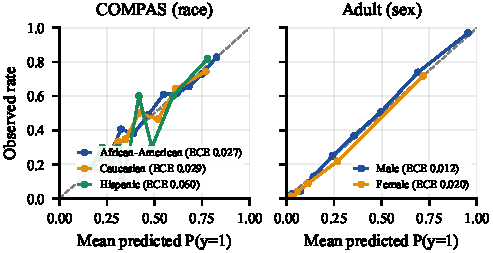
\includegraphics[width=\columnwidth]{figures/calibration.pdf}
\caption{Reliability curves per group (quantile bins, groups with $n\ge30$). The dashed diagonal denotes perfect calibration.}
\label{fig:calib}
\end{figure}

\subsection{Proxies and Explanations}
In Adult, \texttt{relationship} ($I=0.222$) and \texttt{marital\_status} (0.109) are the strongest proxies for sex. In German Credit, after \texttt{personal\_status\_sex} is removed, \texttt{age} (0.047) becomes the top proxy for sex. For COMPAS no single feature is a strong proxy for race, the highest being \texttt{priors\_count} with 0.026. The global SHAP rankings are led by \texttt{priors\_count} and \texttt{age} for COMPAS, \texttt{marital\_status} and \texttt{age} for Adult, and checking account status and loan duration for German Credit. In Adult, \texttt{marital\_status} is the strongest proxy for sex and also the most important feature for the model, which partly explains why a gap of 0.163 remains even after \texttt{sex} is removed.

\subsection{Methodological Pitfalls}\label{sec:pitfalls}
Seven of the bugs we fixed while building FairLens are worth describing, because none of them crashed anything. Each produced a reasonable-looking number, would have passed a test that only checks whether the code runs, and now has its own regression test.

\textbf{P1: Bootstrap-mean inflation.} The average of $|\hat\theta^*|$ over resamples is biased away from zero. Because of this, the dashboard showed DP $=0.043$ for the German Credit baseline, whereas the full-sample value is 0.015, almost three times smaller. We noticed it only because the group selection rates plotted next to it (0.855 and 0.870) were clearly too close for such a gap.

\textbf{P2: Significance on the absolute gap.} For the same German Credit model the interval of the absolute gap, $[0.002, 0.123]$, does not contain zero, which is almost always the case for such intervals. The signed interval $[-0.086, 0.122]$ does contain zero. Putting a fixed cutoff on the absolute interval (for example a lower bound above 0.02) does not fix this.

\textbf{P3: Unseeded randomized classifiers.} Calling \texttt{predict} five times on the same trained COMPAS EG model gave accuracies between 59.3\% and 61.1\%. This spread was more than the 1.1\,pp difference between all the $\eps$ candidates in an earlier sweep. Also, accuracy and fairness were calculated on different random draws, and as EG did not give probabilities, ROC-AUC was silently set to 0.5.

\textbf{P4: Tuning $\eps$ on the test set.} Selecting $\eps$ using test accuracy and test DP leaks information from the test set into a hyperparameter. When the selection was moved to the validation split, the selected $\eps$ changed for COMPAS (0.05 $\to$ 0.01) and Adult (0.005 $\to$ 0.1).

\textbf{P5: Inverted label polarity.} In COMPAS, label~1 stands for recidivism. Our code assumed 1 was the favorable outcome, and as a result it reported the recidivism rate (45.5\%) as the favorable rate (which is actually 54.5\%), treated \emph{low-risk} people as the ones who needed recourse, and asked DiCE to find counterfactuals that \emph{predict} recidivism.

\textbf{P6: Mismatched cached results.} When the default protected attribute was selected, the dashboard showed the stored benchmark results irrespective of the model chosen. For example, Adult with LR showed the DP of the XGBoost baseline (0.163) and not that of LR itself (0.166).

\textbf{P7: Feature-scale mismatch.} LR is trained on standardized features, but local SHAP and DiCE were given the raw features, so their predictions and attributions were wrong. This was fixed by wrapping LR together with its fitted scaler.

Even earlier, the first version had plain leakage (a duplicated label column, and COMPAS score outputs used as features) and reported an F1 of 1.0, which at least looked suspicious. The upload path later showed the same problem in reverse. While testing the dashboard with CSV files we made ourselves, we found that the list of columns dropped as known leakage in the benchmarks was also being applied to uploads, so an ordinary feature that happened to be called \texttt{income} or \texttt{start} disappeared without any warning and accuracy on our test file fell to near chance. Uploads now skip that list. The broader lesson is that an audit pipeline needs tests on the numbers it produces and not only on whether it runs; without them it can overstate the bias, overstate how much of it was removed, or explain the wrong decisions.

\subsection{Limitations}\label{sec:limits}
\textbf{Single-split significance.} The paired bootstrap intervals are from one split. The standard deviations over ten splits in Table~\ref{tab:main} show the variation between splits, but they are not a significance test.

\textbf{Low power on German Credit.} With 200 test rows small disparities cannot be detected, and so a null result on this dataset does not prove that the model is fair.

\textbf{Label bias.} All three datasets contain past decisions which may be biased themselves. In COMPAS, ``recidivism'' actually means re-arrest and not re-offending, and German Credit and Adult were collected decades ago.

\textbf{Deployment constraint.} On the two datasets with significant disparities, Threshold Optimizer gave the best DP--accuracy trade-off, but it requires the protected attribute at prediction time. Using it may not be allowed by law, or the attribute may not be available.

\textbf{Scope.} Only two groups are compared at a time and only one intersection per dataset is studied, so richer subgroup classes~\cite{kearns2018preventing} are not covered. The 5\,pp accuracy limit used for choosing $\eps$ is a policy decision and should ideally be set by domain experts.

%=====================================================================
\section{Conclusion and Future Work}
%=====================================================================
FairLens audits tabular classifiers for group bias, and on three standard benchmarks with ten random splits it gave results that were identical from one run to the next. COMPAS and Adult Income showed large, significant disparities; German Credit showed none that we could call significant with 200 test rows. Where mitigation was needed, Threshold Optimizer lost the least accuracy for the fairness it gained, and the intersectional audits found gaps that single-attribute audits had hidden. For us, though, the most useful outcome was the list of seven errors in our first implementation. Every one of them produced a wrong number that looked right, and we doubt we are the only ones to have made them.

In future, the paired significance tests can be repeated on all ten splits instead of one. We also want to audit more subgroups than a single intersection, use newer datasets with less historical label bias, and try post-processing methods that do not need the protected attribute at prediction time. A user study could also show whether practitioners understand the significance and calibration views of the dashboard as intended.

%=====================================================================
\section*{Contributorship}
%=====================================================================
All authors contributed to the system design, evaluation, and writing of this paper. All authors read and approved the final manuscript.

\balance
\bibliographystyle{IEEEtran}
\bibliography{references}

\end{document}
